%Introduce problem area / give relevant background info
%Introduction - Explain WHY you are doing this study
%Information - Background / your study in the wider context
%Similar work (projects, systems etc.)
%Chapter Summary
	The human species is getting older and older. Our life span is getting longer which means that we have more time to get sick. The longer we live, the more likely it will be that we get one of the chronic diseases. In 2010 there were 759 million people over the age of 60. This was at the time 11 percent of the total population. In 2050 this group is estimated to be more than 2 billion. Not only does the population increase, proportionally the population is getting older and in 2050 it is estimated that 22 percent will be at the age of 60 and older~\cite{UNpub}.\\
	With fewer people taking care of a growing population, new methods needs to be implemented in order to cover the lack of personnel. One of these new methods is home care. If a patient is well enough to care for them self, then it would take a huge burden of the welfare system. A patient who has been living with for example diabetes, knows how to do the daily check up, he knows how to take blood values and know best the state of his illness. If he can live a rich life at home and care for himself he will be happier and it will will free time which can be better spent on patients who need more care.\\
	However, due to the age and progression of the disease of a patient, the health centre might want to keep a closer look at him and do daily check ups. Today this is done by sending a nurse to the home of a patient or by making the patient come to the health centre for daily and weekly check ups. This takes time from both the patient and nurse. If the the patient could send in data regarding their physical status this would greatly reduce the time of health care issues. One method which regards these problem is the Telehealth technology.\\

\subsection{Telehealth}
\label{sub:telehealth}
	Telehealth~\cite{telehealth} is a collection of medical equipment used to monitor and collect data of the patient in his or her home. Data which is collected can be from blood pressure, blood values, weight, surveillance of demented patients or security alarm. The patient can operate the devices and receive daily check ups from the health center.\\

%Skriv mer här

\subsection{Tieto}
\label{sub:tieto}
	Tieto~\cite{tieto} is a Nordic cooperation with its headquarter in Finland. It has 13,720 employers as of the end of 2014. Some of the main focuses of Tieto is cloud driven IT services, healthcare and IT in the industry. One of the fastest growing section of Tieto is Industrial Internet which has a focus of Internet of Things (IoT).\\
	With the need for healthcare services Tieto have, within the section of Industrial Internet, developed a solution which connects the health center with the caretaker so that the caretaker can benefit from being monitored while living in the comfort of ones home. This solution is called Tieto Lifecare.

\subsubsection{Lifecare}
\label{subsub:lifecare}
	Lifecare is a service which is meant to be used all through the life. From child care to family matter and elderly care. Lifecare is used by the health center to monitor patients and by patient to request medical advice. Technically, a router-like device is connected to the internet through a ethernet cable and this router communicates with the different telehealth devices depending on which kind of care the user needs.\\
	With a router connected to the internet by a fixed point in ones home the user will however be bound to the home and limited in his daily life. There is a need to make Tieto Lifecare more mobile.

\subsection{Mobile gateway}
\label{sub:gateway}
	This is the main focus of this thesis, to develop a prototype which takes the functionality of the router and combine this with the mobility of a mobile device such as a phone. To 
	One part of the thesis is to evaluate which OS and producer would be most suitable for making a mobile gateway for Tieto Lifecare.
	
%Skriv mer om existerande lösningar. Continua

\subsubsection{Extended functionality}
\label{subsub:extendedFunc}
	Not only does the mobile gateway make the Tieto Lifecare service more flexible for both the caretaker and the health center. With the built in functionality of today's smart phones, Tieto Lifecare can be extended with more options. Patients with dementia can have their moves tracked if they leave their home, if a patient fall over, then the sensors of the phone can detect this with increased g-force.


\subsection{Continua}
\label{sub:continua}
Continua Alliance is a non-profit organization which works toward generating guidelines for medical equipment used in telehealth. Companies who wish to use the logo provided by Continua must become a member for the organization and then submit their products for testing at a Continua certefied testing laboratory. After all tests has been passed they get a logo which can be used in commercial and adverts for the product.\\
Continua is aiming to become an end to end(E2E) certification to assure that each component in a chain of medical equipment can be interchanged with ease. It is supposed to work with easy plug and play(PnP) standard. If one product is certified, then the next one can be switched by a third without having to change the interface between them.\\
\begin{figure}[]
	\centering
    	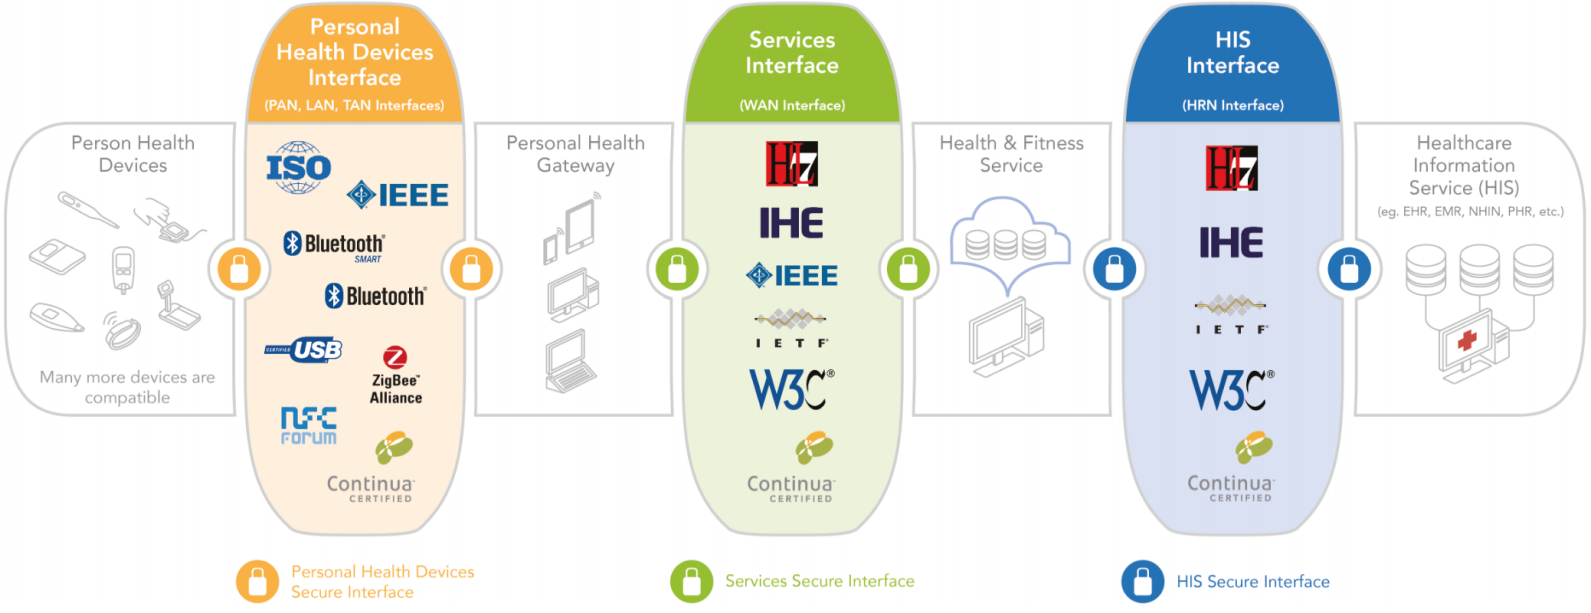
\includegraphics[width=0.9\textwidth]{Pictures/e2eArch}
		\caption{Continua E2E Architecture}
		Source: \href{http://www.continuaalliance.org/}{Continua Health Alliance}
	\label{fig:e2eArch}
\end{figure}
	In figure~\ref{fig:e2eArch} the E2E architecture of continua is shown. At the left end there is the personal health devices(PHD) which includes scales, thermometers, blood pressure measurement device and so forth. These devices is connected to a aggregation device, shown as a personal health gateway(PHG) in the figure. The interface between the PHD and PHG depends on which kind of device. It can be three kinds of interfaces~\cite{tanpanlan}. Touch  area network(TAN-IF), personal area network(PAN-IF) and local area network(LAN-IF).\\
	The link between the PHG and the health and fitness service(HFS) is defined by the wide area network interface(WAN-IF)~\cite{wan-if}. If the PHD connected to a PHG is regarded as a front-end, then the HFS is regarded as the back-end of the E2E solution. The HFS communicates with both the PHG and with the health center. This is however out of the scope of this thesis which will cover a new PHG solution.\\
	Between the PHD and PHG the Continua guidelines are based on the ISO/IEEE standard: 11073-10. Between the PHG and HFS, the guideline are based on the IHE PCD-01 Transaction: Communicate PCD Data. More about this in section~\ref{subsub:ieee11073}~and~\ref{subsub:ihepcd01}

\subsubsection{ISO/IEEE 11073}
\label{subsub:ieee11073}
	Continua dictates that the standard being used for data transfer between the PHD and PHG is the one defined by ISO/IEEE 11073. This standard have been tested and implemented by all manufacturers who wish to continua-certificate their devices. 
	
	Antidote


\subsubsection{IHE PCD-01}
\label{subsub:ihepcd01}

\subsubsection{Android BluetoothHealth}
\label{subsub:bthealth}

\subsection{Chapter Summary}
\label{sub:backSum}
%-1. 38880358	6. 39701424
%2. 53984474	7. 55749974
%3. 32169561	8. 84597658
%4. 03891758	9. 34978594
%5. 51124190	 
